% Created 2015-06-11 Thu 09:14
\documentclass[presentation]{beamer}
\usepackage[utf8]{inputenc}
\usepackage[T1]{fontenc}
\usepackage{fixltx2e}
\usepackage{graphicx}
\usepackage{longtable}
\usepackage{float}
\usepackage{wrapfig}
\usepackage{rotating}
\usepackage[normalem]{ulem}
\usepackage{amsmath}
\usepackage{textcomp}
\usepackage{marvosym}
\usepackage[integrals]{wasysym}
\usepackage{amssymb}
\usepackage{hyperref}
\tolerance=1000
\usepackage{minted}
\usepackage{amsmath}
\usepackage{tikz}
\usepgflibrary{shapes.geometric}
\usetikzlibrary{calc}
\usetikzlibrary{positioning}
\usetikzlibrary{intersections,decorations.pathreplacing,shapes,arrows}
\usetikzlibrary{plotmarks}
\usepackage{amsmath,amssymb}
\usepackage{mathtools}
\DeclareMathOperator{\tr}{tr}
\usepackage{pgfplots}
\subtitle{solving equations by writing them down}
\institute{Departments of Computing and Mathematics, Imperial College London}
\renewcommand{\vec}{\mathbf}
\usetheme{IC}
\author{Lawrence Mitchell}
\date{Thursday 11th June 2015}
\title{From symbolic to numerical computing}
\hypersetup{
  pdfkeywords={},
  pdfsubject={},
  pdfcreator={Emacs 24.4.91.1 (Org mode 8.2.7b)}}
\begin{document}

\maketitle
\begin{frame}{Outline}
\tableofcontents
\end{frame}



\section{Introduction}
\label{sec-1}

\begin{frame}[label=sec-1-1]{Numerical simulation}
\begin{itemize}
\item Computer simulation at the heart of swathes of modern science and
engineering:

\begin{itemize}
\item Car, aircraft, building design
\item Reactor modelling
\item Weather prediction
\item Climate modelling
\item Drug design
\item Traffic planning
\item \ldots{}
\end{itemize}
\end{itemize}
\end{frame}

\begin{frame}[label=sec-1-2]{Numerical solution of PDEs}
\begin{enumerate}
\item Write down the equations you'd like to solve.  Find $u$ s.t.
$F(u) = 0$
\item Select appropriate \emph{discrete} approximation.  Find $u_h$ s.t.
$F_h(u_h) = 0$
\item Implement on computer
\item \ldots{}
\item Profit!
\end{enumerate}
\end{frame}

\section{Solution strategies}
\label{sec-2}

\begin{frame}[label=sec-2-1]{The finite element method}
\begin{itemize}
\item Consider PDE $F(u) = 0 \quad \text{in}\:\Omega$
\item Seek \emph{weak} solution in some space of functions $V$.  Find $u\in
  V$ s.t.
\end{itemize}
\begin{equation*}
\int_\Omega \!F(u) v\, \mathrm{d}x = 0 \quad \forall v \in V
\end{equation*}
\begin{itemize}
\item Choose discrete $V_h \subset V$, and seek $u_h \in V_h$.
\item Pick \emph{basis} for $V_h$
\end{itemize}
\begin{tikzpicture}[remember picture, overlay]
\node[yshift=-8cm,xshift=-2cm] at (current page.north east)
{\begin{tikzpicture}[remember picture, overlay]
    \draw (0, 0) -- (1, 0) -- (1, 2) -- (-1, 2) -- (0, 1) -- cycle;
\end{tikzpicture}
};
\end{tikzpicture}
\end{frame}

\begin{frame}[label=sec-2-2]{FEM II}
\begin{itemize}
\item Divide domain $\Omega$ into elements $E$
\item Integrals become sums of integrals over elements
\begin{itemize}
\item Same for all problems
\end{itemize}
\end{itemize}
\begin{equation*}
\int_\Omega\! F(u_h) v_h \, \mathrm{d}x = \sum_{e \in E} \int_e\! F(u_h)v_h\, \mathrm{d}x
\end{equation*}
\begin{itemize}
\item Perform element integrals with numerical quadrature
\begin{itemize}
\item Different for each problem
\item Variability in innermost loop
\end{itemize}
\item Can we
\begin{enumerate}
\item Express problem in succinct way mimicing maths?
\item Still achieve good performance?
\end{enumerate}
\end{itemize}

\begin{tikzpicture}[remember picture, overlay]
\node[yshift=-4cm,xshift=-2cm] at (current page.north east)
{\begin{tikzpicture}[remember picture, overlay]
    \draw (0, 0) -- (0, 1) -- (1, 0) -- (1, 2) -- (-1, 2) -- (0, 1) --
    (1, 2) (0, 0) -- (1, 0);
\end{tikzpicture}
};
\end{tikzpicture}
\end{frame}
\section{Automated numerical computing}
\label{sec-3}

\begin{frame}[fragile,label=sec-3-1]{Poisson equation}
 \begin{columns}
\begin{column}{0.45\textwidth}
\begin{block}{PDE}

\begin{itemize}
\item Solve $\nabla^2 u = 1$ in $\Omega$, $u=0$ on $\partial\Omega$.
\item Weak formulation.  Find $u \in V$ s.t.
\end{itemize}
\begin{equation*}
-\langle\nabla u, \nabla v\rangle = \langle 1, v \rangle \quad \forall v \in V
\end{equation*}

\visible<2->{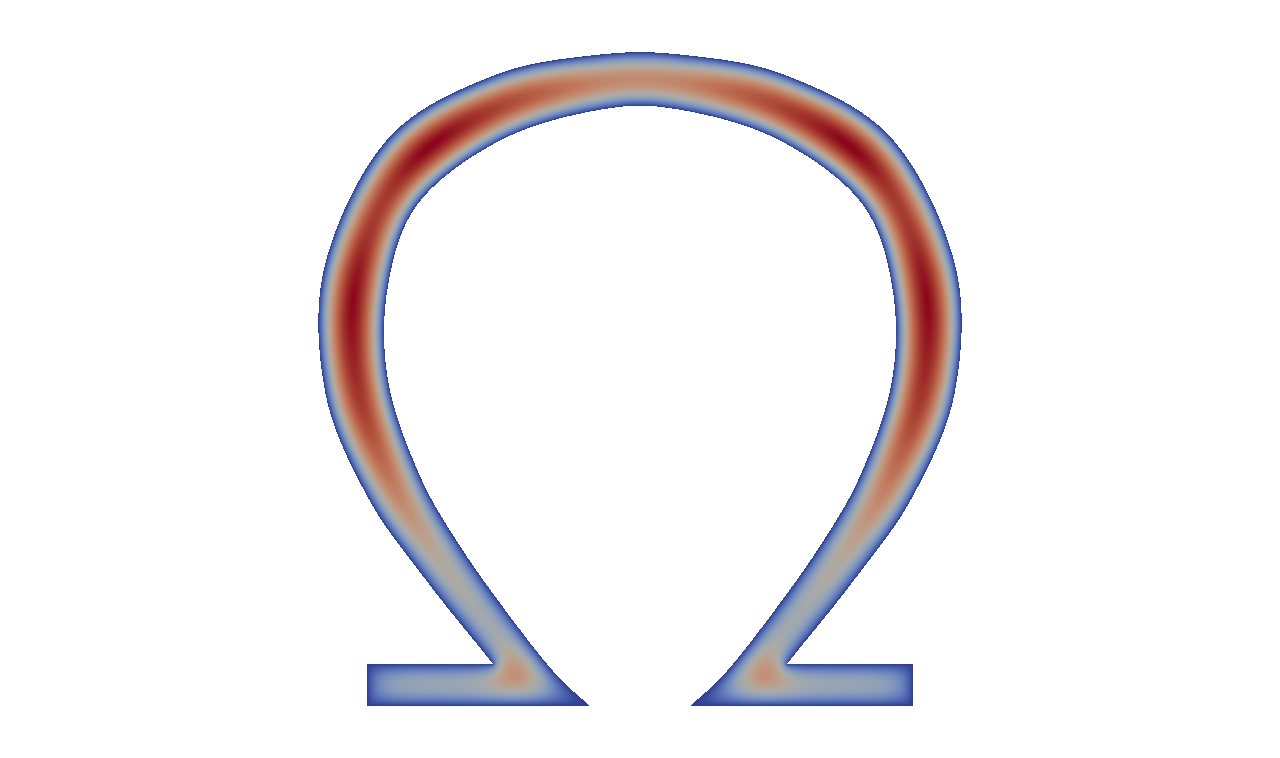
\includegraphics[height=0.4\textheight]{06-10-Imperial-RA-symposium-firedrake.figures/poisson-omega}}
\end{block}
\end{column}
\begin{column}{0.55\textwidth}
\begin{block}{Code}

\begin{minted}[frame=none,xleftmargin=1em,xrightmargin=1em,fontsize=\scriptsize,mathescape]{python}
from firedrake import *
mesh = Mesh("omega.msh")
V = FunctionSpace(mesh, "CG", 2)
u = TrialFunction(V)
v = TestFunction(V)
f = Function(V)
bc = DirichletBC(V, 0, "boundary")
sol = Function(V)
a = -dot(grad(u), grad(v))*dx
L = f*v*dx
solve(a == L, sol, bcs=bc)
\end{minted}
\end{block}
\end{column}
\end{columns}
\end{frame}

\begin{frame}[fragile,label=sec-3-2]{What's going on}
 \begin{itemize}
\item Use DSLs to provide correct levels of abstraction

\item Symbolic representation of equations using \emph{Unified Form Language}
  Alnæs et al., \verb~arxiv: 1211.4047 [cs.MS]~
\begin{itemize}
\item DSL for finite element variational forms embedded in Python
\item Part of the FEniCS project \url{http://www.fenicsproject.org}
\end{itemize}

\item FEniCS form compiler converts to low-level implementation of element
integral ("kernel")

\item Marshalling of assembly of operators and solving performed by
Firedrake system \verb~arxiv: 1501.01809 [cs.MS]~ and \verb~arxiv: 1411.2940 [math.NA]~
\begin{itemize}
\item \url{http://www.firedrakeproject.org}
\end{itemize}
\end{itemize}
\end{frame}

\begin{frame}[label=sec-3-3]{Symbolic manipulation is powerful}
\begin{itemize}
\item For nonlinear problems need \emph{linearisation} around current solution
\begin{itemize}
\item traditional AD tools can give you this, but \emph{slow}
\item Instead, do AD on symbolic objects, and generate efficient code
\end{itemize}
\item Sensitivity analysis needs adjoint
\begin{itemize}
\item time runs backwards: need linearisation around forward trajectory
\end{itemize}
\item Minimisation problems need gradients
\end{itemize}
\end{frame}

\begin{frame}[fragile,label=sec-3-4]{Code generation}
 \begin{itemize}
\item Many options for efficient evaluation of element kernels
\begin{itemize}
\item No one best solution
\end{itemize}
\item \emph{Generation} from high-level description can explore space of
possible transformations
\begin{itemize}
\item Ølgaard and Wells, \verb~arxiv: 1104.0199 [cs.MS]~
\item Luporini et al., \verb~arxiv: 1407:0904 [cs.MS]~
\end{itemize}
\end{itemize}
\end{frame}

\begin{frame}[label=sec-3-5]{Tieing global data structures together}
\begin{itemize}
\item Element kernel acts on local data
\item Global execution is:
\begin{itemize}
\item \emph{gather} from global to local
\item \emph{compute} on local data
\item \emph{scatter} result to global data
\end{itemize}
\item access \emph{stencil} defined by mesh connectivity
\end{itemize}
\end{frame}

\begin{frame}[label=sec-3-6]{Parallel loops over mesh entities}
\begin{itemize}
\item The "go do that everywhere" step suggests an iteration abstraction
\item PyOP2 is a python library realising this idea
\begin{itemize}
\item \url{http://github.com/OP2/PyOP2}
\end{itemize}
\item Core concepts:
\begin{description}
\item[{\emph{Sets}}] iterable entities
\item[{\emph{Dats}}] abstract managed arrays (data defined on a set)
\item[{\emph{Maps}}] relationships between elements of sets
\item[{\emph{Kernels}}] the "local" computation
\item[{\emph{parallel loop}}] Data parallel iteration over a set
\end{description}
\item Arguments to parallel loop indicate how to gather/scatter global
data using \emph{access descriptors}
\end{itemize}
\end{frame}

\begin{frame}[label=sec-3-7]{A picture}
\begin{center}
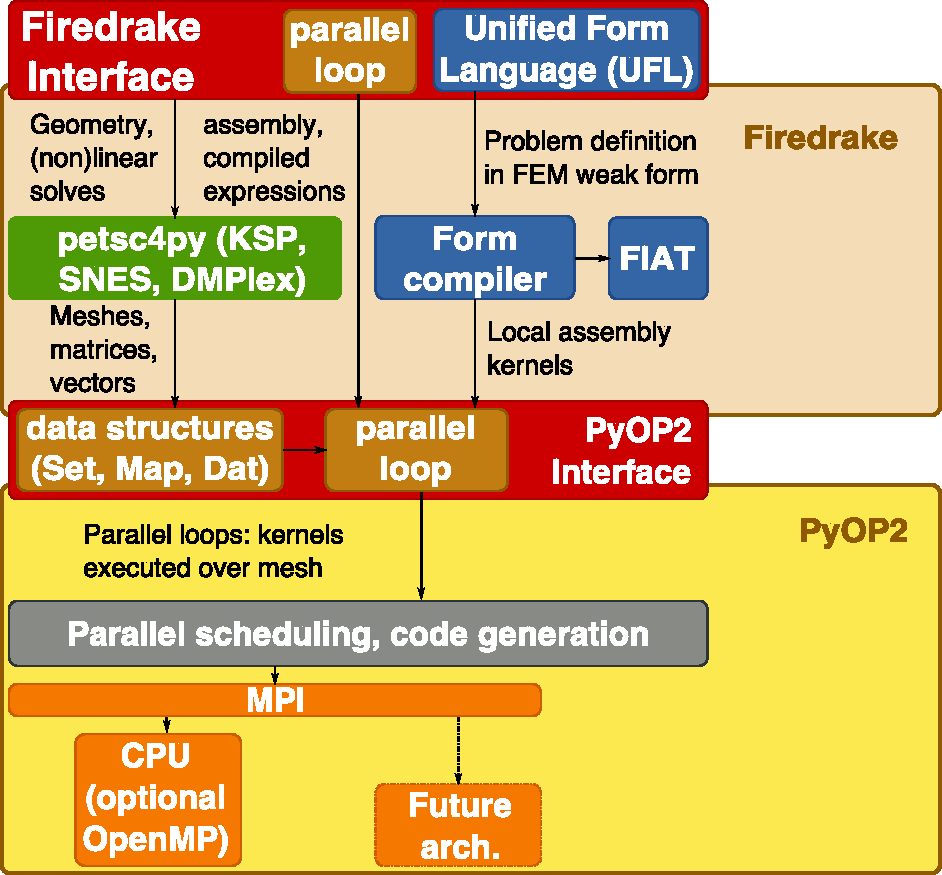
\includegraphics[height=0.9\textheight]{06-10-Imperial-RA-symposium-firedrake.figures/toolchain}
\end{center}
\end{frame}

\section{Some movies}
\label{sec-4}

\begin{frame}[label=sec-4-1]{Incompressible Navier-Stokes}
\begin{equation*}
\begin{aligned}
\frac{\partial \vec{u}}{\partial t} + \underbrace{(\vec{u} \cdot \nabla)\vec{u}}_{\mathclap{\text{Convection}}} &= 
     \overbrace{-\nabla p}^{\mathclap{\text{Internal source}}} + \underbrace{\nu \nabla^2 \vec{u}}_{\mathclap{\text{Diffusion}}} & \text{Momentum conservation}\\
\nabla \cdot \vec{u} &= 0 & \text{Mass conservation}
\end{aligned}
\end{equation*}

\begin{center}
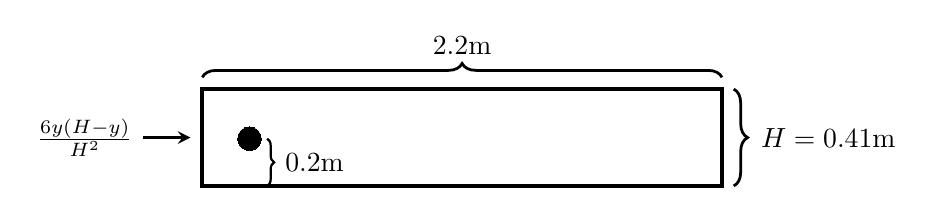
\begin{tikzpicture}[line width=1.5pt, line join=miter,scale=3]
\draw (0, 0) -- (0, 0.41) -- (2.2, 0.41) -- (2.2, 0) -- cycle;
\draw[fill,line width=0pt] (0.2,0.2) circle[radius=0.05];
\draw[-stealth, line width=1pt] (-0.25, 0.205) node[left] (text) {$\frac{6y(H-y)}{H^2}$} -- +(0.2, 0);

\draw[decorate, decoration={brace, amplitude=5pt, mirror}, line width=1pt, xshift=0.05cm] (2.2, 0) -- (2.2, 0.41) node [midway, xshift=1.2cm] {$H = 0.41\text{m}$};
\draw[decorate, decoration={brace, amplitude=5pt}, line width=1pt, yshift=0.05cm] (0, 0.41) -- (2.2, 0.41) node [midway, yshift=0.4cm] {$2.2\text{m}$};
\draw[decorate, decoration={brace, amplitude=2.5pt, mirror}, line width=0.8pt] (0.275, 0) -- (0.275, 0.2) node [midway, xshift=0.6cm] {$0.2\text{m}$};
\end{tikzpicture}
\end{center}
\begin{itemize}
\item $\vec{u} = \vec{0}$ on side walls, $p = 0$ at exit
\item Kinematic viscosity, $\nu = 2\times10^{-4}$.  $\text{Re}\approx1200$
\end{itemize}
\end{frame}


\begin{frame}[label=sec-4-2]{Vortex shedding}
\end{frame}


\begin{frame}[label=sec-4-3]{Phase separation}
\begin{block}{The Cahn-Hilliard equation}
\begin{itemize}
\item Model of phase separation in binary fluids
\end{itemize}
\begin{equation*}
\begin{aligned}
F[\phi(x, t)] &= \int \overbrace{\alpha \phi^2 + \beta \phi^4 + \epsilon}^{\mathclap{\text{Landau potential}}} + \underbrace{\frac{\gamma}{2} |\nabla\phi|^2}_{\mathclap{\text{interface penalty}}}\,\mathrm{d}x & \text{Free energy}\\
\mu = \frac{\delta F}{\delta \phi} &= 2\alpha\phi + 4\beta\phi^3 - \gamma\nabla^2\phi & \text{Chemical potential}\\
\frac{\partial \phi}{\partial t} &= \nabla \cdot D(\phi) \nabla \mu & \text{Continuity}
\end{aligned}
\end{equation*}
\end{block}
\end{frame}

\begin{frame}[label=sec-4-4]{Phase separation}
\begin{block}{Weak formulation}
\begin{itemize}
\item Choose a square domain $\Omega = [0, 1] \times [0, 1]$
\item Crank-Nicholson timestepping
\item Random initial $\phi$
\item Find $\phi, \mu \in V \times V \subset H^1 \times H^1$ such that
\end{itemize}
\begin{equation*}
\begin{aligned}
\langle \phi^{n+1} - \phi^n, q \rangle + \Delta t D \langle \nabla ((1 - \theta)\mu^{n} + \theta \mu^{n+1}), \nabla q \rangle &= 0 \quad \forall\, q \in V\\
\langle \mu - \partial_\phi f, v \rangle - \gamma \langle \nabla \phi, \nabla v \rangle &= 0 \quad \forall\, v \in V\\
n\cdot\nabla \phi = n\cdot\nabla \mu &= 0 \quad\text{on $\partial\Omega$}
\end{aligned}
\end{equation*}

\begin{tikzpicture}[remember picture, overlay]
\node at (9.5, 3.5) {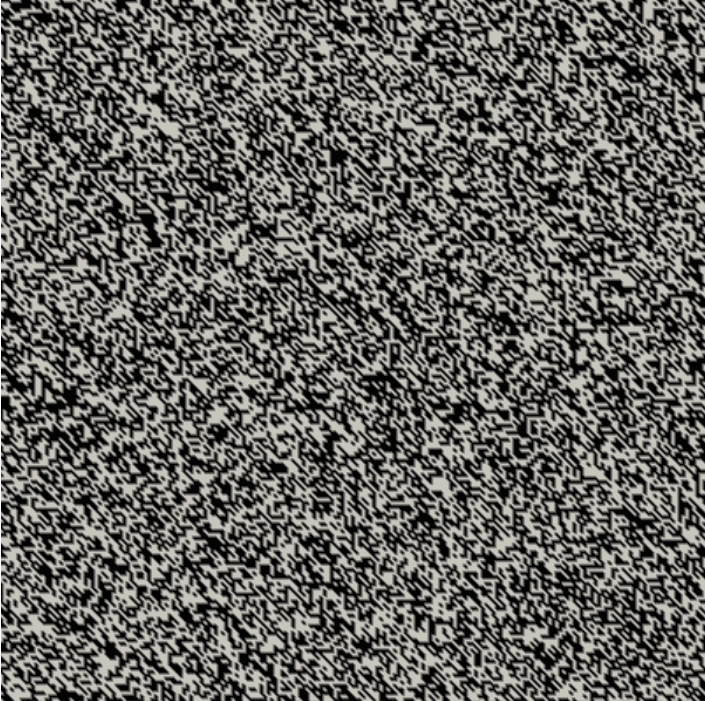
\includegraphics[width=2.5cm]{06-10-Imperial-RA-symposium-firedrake.figures/phase-initial}};
\end{tikzpicture}
\end{block}
\end{frame}
\begin{frame}[fragile,label=sec-4-5]{Code}
 \begin{minted}[frame=none,xleftmargin=1em,xrightmargin=1em,fontsize=\scriptsize,mathescape]{python}
mesh = UnitSquareMesh(100, 100)
V = FunctionSpace(mesh, "CG", 1)
W = V*V
gamma = Constant(0.005)
D = Constant(10)
q, v = TestFunctions(W)
u = Function(W)
u0 = Function(W)
phi, mu = split(u)
phi0, mu0 = split(u0)
phi = variable(phi)
f = 10*(phi**2 - 1)**2
dfdphi = diff(f, phi)
theta = 0.5
mu_theta = (1-theta)*mu0 + theta*mu
dt = 5e-6
F = ((phi - phi0)*q + dt*D*dot(grad(mu_theta), grad(q)) + 
     (mu - dfdphi)*v - gamma*dot(grad(phi), grad(v)))*dx
for _ in range(200):
    u0.assign(u)
    solve(F == 0, u)
\end{minted}
\end{frame}

\begin{frame}[label=sec-4-6]{And finally\ldots{}}
\begin{itemize}
\item All code freely available
\begin{description}
\item[{Firedrake}] firedrakeproject.org
\item[{PyOP2}] github.com/OP2/PyOP2
\end{description}

\item A cast of tens
\begin{description}
\item[{People}] firedrakeproject.org/team.html
\item[{Funding}] firedrakeproject.org/funding.html
\end{description}

\item For another, broader view
\begin{itemize}
\item Anders Logg \emph{Implementing mathematics: domain specific languages and automated computing}
\item Tuesday 30th June at 16:10 in Huxley 311
\end{itemize}
\end{itemize}
\end{frame}
% Emacs 24.4.91.1 (Org mode 8.2.7b)
\end{document}
